\newpage\setcounter{section}{8}
\section{Integral Curves and Flows}

The primary objects associated with smooth vector fields are \textit{integral curves}, which are smooth curves whose velocity at each point is equal to the value of the vector field there. The collection of all integral curves of a given vector field on a manifold determines a family of diffeomorphism of (open subsets of) the manifold called a \textit{flow}. In applied mathematics, these objects are often used to approximate solutions to differential equations. The methodology for doing this will become more clear as we discuss the fundamental theorem on flows.

\subsection{Integral Curves and Flows}\nl

\dfng Suppose $M$ is a smooth manifold \wowob. If $V$ is a vector field on $M$, an \df{integral curve of V} is a differentiable curve $\ga:J\ra M$ whose velocity at each point is equal to the value of $V$ at that point:
\[\ga\p(t) = V_{\ga(t)}\quad\text{for all }t\in J.\]
If $0\in J$, the point $\ga(0)$ is called the \df{starting point of $\boldsymbol{\ga}$}.

\begin{center}
    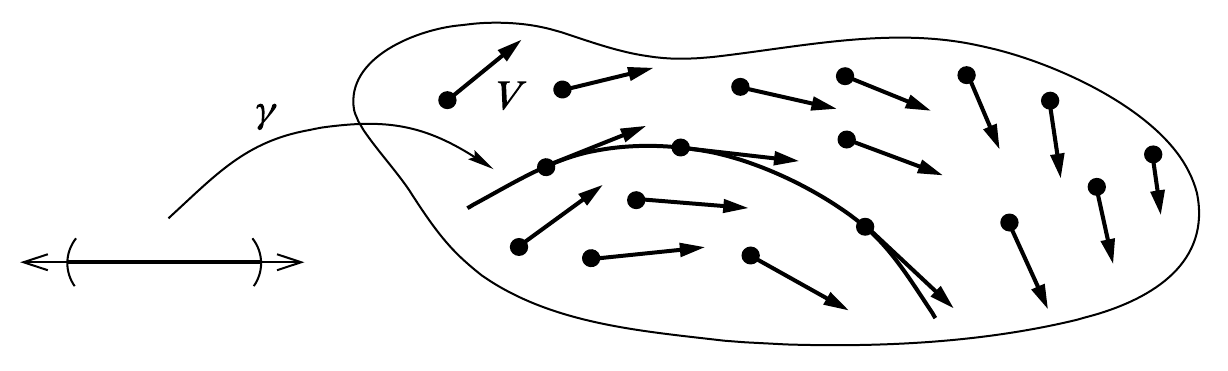
\includegraphics[scale = 0.3]{chapter09/c9f1.png}
\end{center}

\setcounter{thm}{1}

\begin{prop}
Let $V$ be a smooth vector field on a smooth manifold $M$. For each point $p\in M$, there exists $\vep > 0$ and a smooth curve $\ga(-\vep, \vep)\ra M$ that is an integral curve of $V$ starting at $p$.
\end{prop}


\begin{lem}[Rescaling Lemma]
Let $V$ be a smooth vector field on a smooth manifold $M$, let $J\seq \R$ be an interval, and let $\ga:J\ra M$ be an integral curve of $V$. For any $a\in \R$, the curve $\td\ga:\td J\ra M$ defined by $\td\ga(t) = \ga(at)$ is an integral curve of the vector field $aV$, where $\td J = \{t\ :\ at \in J\}$.
\end{lem}

\begin{lem}[\hlb{Translation Lemma}]
Let $V, M, J$ and $\ga$ be as in the preceding lemma. For any $b\in \R$, the curve $\wh\ga:\wh J\ra M$ defined by $\wh\ga(t) = \ga(t + b)$ is also an integral curve of $V$, where $\wh J = \{t\ :\ t + b \in J\}$.
\end{lem}

\begin{prop}[Naturality of Integral Curves]
Suppose $M$ and $N$ are smooth manifold and $F:M\ra N$ is a smooth map. Then $X\in \fkX(M)$ and $Y\in \fkX(N)$ are $F$-related if and only if $F$ tales integral curve so of $X$ to integral curves of $Y$, meaning that for each integral curve of $X$, $F\circ \ga$ is an integral curve of $Y$.
\end{prop}

\dfn We define a \df{global flow} on $M$ (also called a \df{one-parameter group action}) to be a continuous left $\R$-action on $M$; that is, a continuous map $\theta:\R\x M\ra M$ satisfying the following properties for all $s,t\in \R$ and $p\in M$:
\[\theta(t,\theta(s,p)) = \theta(t + x, p),\qquad \theta(0,p) = p.\]

\dfn Given a global flow $\theta$ on $M$, we define two collections of maps as follows:
\begin{itemize}
    \item For each $t\in \R$, define a continuous map $\theta_t:M\ra M$ by 
    \[\theta_t(p) = \theta(t,p).\]
    \item For each $p\in M$, define a curve $\theta^{(p)}:\R\ra M$ by 
    \[\theta^{(p)}(t) = \theta(t,p).\]
\end{itemize}

\dfn If $\theta:\R\x M\ra M$ is a smooth global flow, for each $p\in M$ we define a tangent vector $V_p\in T_pM$ by 
\[V_p = \theta^{(p)\prime}(0).\]
The assignment $p\mapsto V_p$ is a (rough) vector field om $M$, which is called the \df{infinitesimal generator of $\boldsymbol{\theta}$}.

\setcounter{thm}{6}

\begin{prop}
Let $\theta:\R\x M\ra M$ be a smooth global flow on a smooth manifold $M$. The infinitesimal generator $V$ of $\theta$ is a smooth vector field on $M$, and \hl{each curve $\theta^{(p)}$ is an integral curve of $V$.}
\end{prop}

\begin{center}
    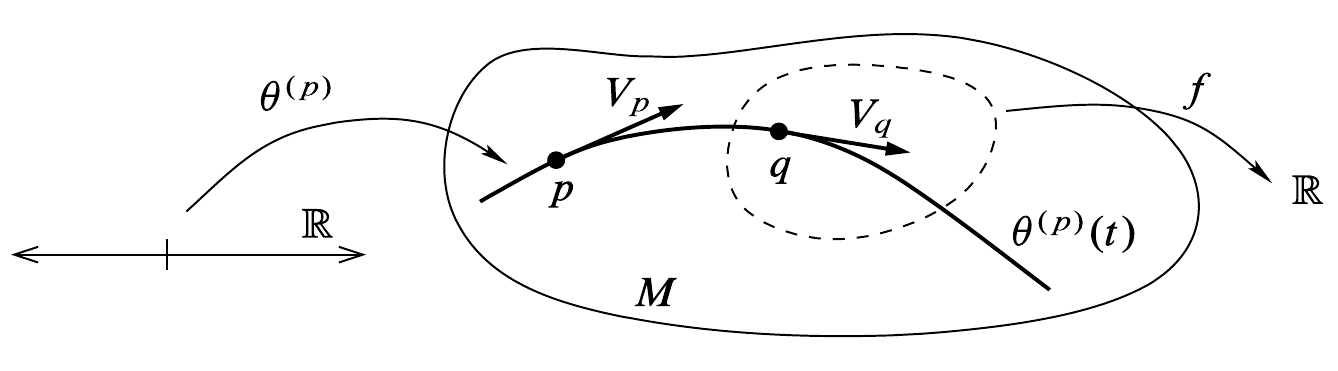
\includegraphics[scale = 0.3]{chapter09/c9f4.png}
\end{center}

\setcounter{thm}{8}

\begin{ex}[Smooth Vector Field that does not Generate a Smooth Global Flow]
Let $M = \R^2\backslash\{0\}$ with standard coordinates $(x,y)$, and let $V$ be the vector field $\pdd{x}$ on $M$. The unique integral curve of $V$ starting at $(-1,0)\in M$ is $\ga(t) = (t - 1, 0)$. However, in this case, $\ga$ cannot be extended continuously past $t = 1$. This is intuitively evident because of the "hole" in $M$ at the origin.
\end{ex}

\dfn If $M$ is a manifold, a \df{flow domain} for $M$ is an open subset $\DD\seq \R\x M$ with the property that for each $p\in M$, the set $D^{(p)} = \{t\in \R\ :\ (t,p)\in \DD\}$ is an open interval containing 0.

\dfn A \df{flow} (or \df{local flow}) on $M$ is a continuous map $\theta:\DD\ra M$, where $\DD\seq \R\x M$ is a flow domain, that satisfies the following group laws: for all $p\in M$
\[\theta(0,p) = p,\]
and for all $s\in \DD^{(p)}$ and $t\in \DD^{(\theta(s,p))}$ such that $s + t \in \DD^{(p)}$,
\[\theta(t,\theta(s,p)) = \theta(t + x, p).\]

\begin{center}
    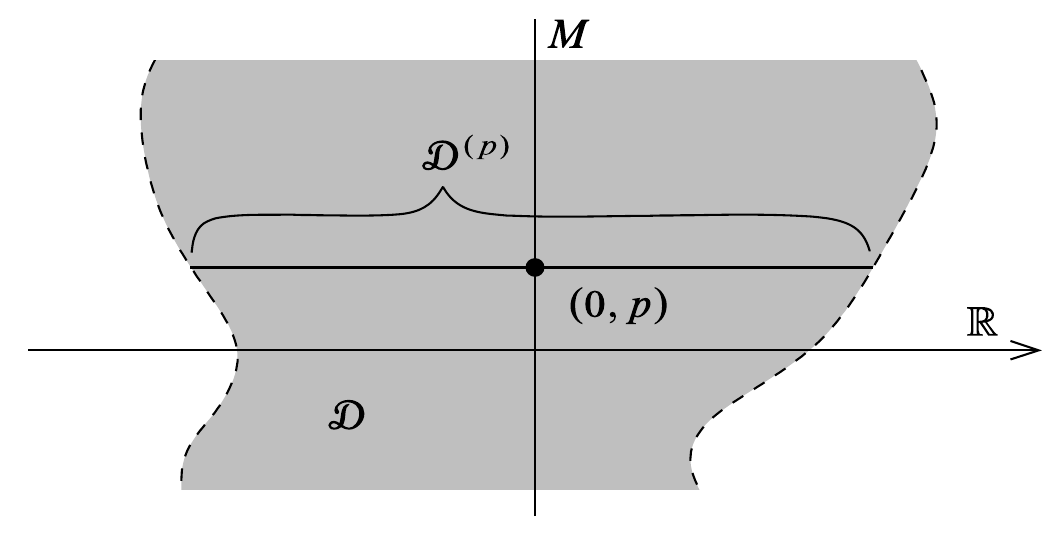
\includegraphics[scale = 0.3]{chapter09/c9f5.png}
\end{center}

\dfn If $\theta$ is a flow, we define $\theta_t(p) = \theta^{(p)} = \theta(t,p)$ whenever $(t,p)\in \DD$. For each $t\in \R$, we also define
\[M_t = \{p\in M\ :\ (t,p)\in \DD\},\]
so that 
\[p\in M_t\Leftrightarrow t\in \DD^{(p)}\Leftrightarrow (t,p)\in \DD.\]
If $\theta$ is smooth, the \df{infinitesimal generator of $\boldsymbol{\theta}$} is defined by $V_p = \theta^{(p)\prime}(0)$.

\setcounter{thm}{10}

\begin{prop}
If $\theta:\DD\ra M$ is a smooth flow, then the infinitesimal generator $V$ of $\theta$ is a smooth vector field, and each cure $\theta^{(p)}$ is an integral curve of $V$.
\end{prop}

\dfn A \df{maximal integral curve} is one that cannot be extended to an integral curve on any larger open interval, and a \df{maximal flow} is a flow that admits no extension to a flow on a larger flow domain.

\begin{thm}[\hlb{Fundamental Theorem on Flows}]
Let $V$ be a smooth vector field on a smooth manifold $M$. There is a unique smooth maximal flow $\theta:\DD\ra M$ whose infinitesimal generator is $V$. This flow has the following properties:
\begin{enumerate}
    \item For each $p\in M$, the curve $\theta^{(p)}:\DD^{(p)}\ra M$ is the unique maximal integral curve of $V$ starting at $p$.
    \item If $s\in \DD^{(p)}$, then $\DD^{(\theta(s,p))}$ is the interval $\DD^{(p)} - s = \{t - s\ :\ t\in \DD^{(p)}\}$.
    \item For each $t\in \R$, the set $M_t$ is open in $M$, and $\theta_t:M_t\ra M_{-t}$ is a diffeomorphism with inverse $\theta_{-t}$.
\end{enumerate}
\end{thm}

\dfn We say that a smooth vector field is \df{complete} if it generates a global flow, or equivalently if each of its maximal integral curves is defined for all $t\in \R$.

\setcounter{thm}{14}

\begin{lem}[\hlb{Uniform Time Lemma}]
Let $V$ be a smooth vector field on a smooth manifold $M$, and let $\theta$ be its flow. Suppose there is a positive number $\vep$ such that for every $p\in M$, the domain $\theta^{(p)}$ contains $(-\vep,\vep)$. Then $V$ is complete.
\end{lem}

\begin{thm}
Every compactly supported smooth vector field on a smooth manifold is complete.
\end{thm}

\begin{cor}
On a compact smooth manifold, every smooth vector field is complete
\end{cor}

\begin{thm}
\hl{Every left-invariant vector field on a Lie group is complete.}
\end{thm}

\begin{thm}[\hl{Flowout Theorem}]
Suppose $M$ is a smooth manifold, $S\seq M$ is an embedded $k$-dimensional submanifold, and $V\in \fkX(M)$ is a smooth vector field that is nowhere tangent to $S$. Let $\theta\DD\ra M$ be the flow of $V$, let $\OO = (\R\x S)\cap \DD$ and let $\Phi = \theta|_\OO$.
\begin{enumerate}
    \item $\Phi:\OO\ra M$ is an immersion.
    \item $\pdd{t}\in \fkX(\OO)$ is $\Phi$-related to $V$.
    \item There exists a smooth positive function $\de:S\ra \R$ such that the restriction of $\Phi$ to $\OO_\de$ is injective, where $\OO_\de\seq \OO$ is the flow domain 
    \[\OO_\de = \{(t.p)\in \OO\ :\ |t| < \de(p)\}.\]
    Thus, $\Phi(\OO_\de)$ is an immersed submanifold of $M$ containing $S$, and $V$ is tangent to this submanifold.
    \item If $S$ has codimension 1, then $\Phi|_{\OO_\de}$ is a diffeomorphism onto an open submanifold of $M$.
\end{enumerate}
\end{thm}

\dfn The submanifold $\Phi(\OO_\de)\seq M$ in the previous theorem is called a \df{flowout from S along V}.

\dfng If $V$ is a vector field on $M$, a point $p\in M$ is said to be a \df{singular point of V} if $V_p = 0$, and a \df{regular point} otherwise.

\setcounter{thm}{20}

\begin{prop}
Let $V$ be a smooth vector filed on a smooth manifold $M$, and let $\theta:\DD\ra M$ be the flow generated by $V$. If $p\in M$ is a singular point of $V$, then $\DD\op = \R$ and $\theta\op$ is the constant curve $\theta\op(t)\equiv p$. If $p$ is a regular point, then $\theta\op:\DD\op\ra M$ is a smooth immersion.
\end{prop}

\begin{thm}[\hlb{Canonical Form Near a Regular Point}]
Let $V$ be a smooth vector field on a smooth manifold $M$, and let $p\in M$ be a regular point of $V$. There exist smooth coordinates $(s^i)$ on some neighborhood of $p$ in which $B$ has the coordinate representation $\pdd{s^1}$. If $S\seq M$ is any embedded hypersurface (submanifold with codimension 1) with $p\in S$ and $V_P\nin T_pS$, then the coordinates can also be chosen so that $s^1$ is a local defining function for $S$.
\end{thm}


\begin{ex}
Let $W = x\pdd{y} - y\pdd{x}$ on $\R^2$. The flow of $W$ is given by 
\[\theta_t(x,y) = (x\cos(t) - y\sin(t), x\sin(t) + y\cos(t).\]
The point $(1,0)\in \R^2$ is a regular point of $W$ because $W_{(1,0)} = \ev{\pdd{y}}{(1,0)}\neq 0$. Because $W$ has nonzero $y$-coordinate there, we can take $S$ to be the $x$-axis, parameterized by $X(s) = (s,0)$. We define $\Psi:\R^2\ra R^2$ by 
\[\Psi(t,s) = \theta_t(s,0) = (s\cos(t), s\sin(t)),\]
and then solve locally for $(t,s)$ in terms of $(x,y)$ to obtain the following coordinate map in a neighborhood of $(1,0)$:
\[(t,s) = \Psi\inv(x,y) =\lp \tan\inv\lp\frac{y}{x}\rp,\sqrt{x^2 + y^2}\rp.\]
It is easy to check that $W = \pdd{t}$ in these coordinates.
\end{ex}



\subsection{Lie Derivatives}\nl

\dfn Let $M$ be a smooth manifold, $V$ a smooth vector field on $M$, and $\theta$ the flow of $V$. For any smooth vector field $W$ on $M$, define a rough vector field on $M$, denoted by $\LL_V W$ and called the \df{Lie derivative of W with respect to V}, by 
\begin{align*}
    (\LL_V W)_p &= \ev{\frac{d}{dt}}{t = 0}d(\theta_{-t})_{\theta_t(p)}(W_{\theta_t(p)})\\
    &=\lim_{t\ra 0} \frac{d(\theta_{-t})_{\theta_t(p)}(W_{\theta_t(p)}) - W_p}{t},
\end{align*}
provided the derivative exists.

\begin{center}
    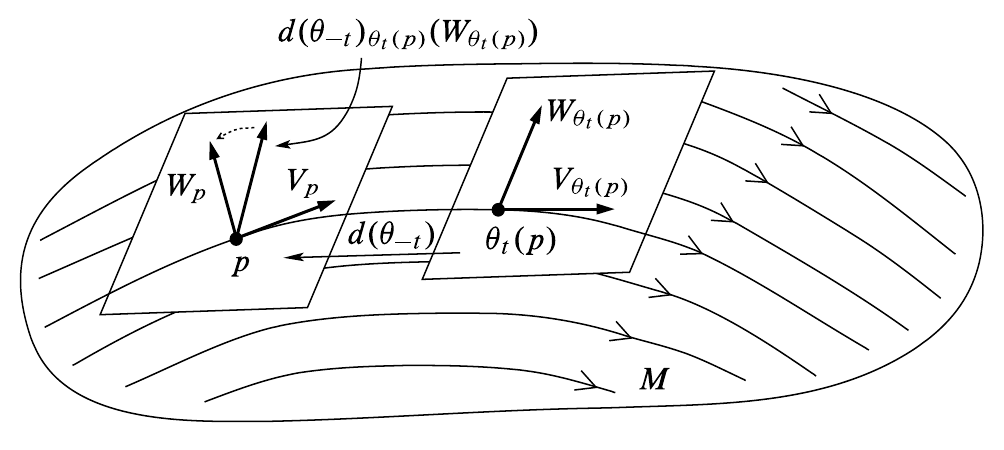
\includegraphics[scale = 0.38]{chapter09/c9f13.png}
\end{center}

\setcounter{thm}{35}

\begin{lem}
Suppose $M$ is a smooth manifold \wowob, and $V,W\in \fkX(M)$. If $\bd M\neq \es$, assume in addition that $V$ is tangent to $\bd M$. Then $(\LL_pW)_p$ exists for every $p\in M$, and $\LL_V W$ is a smooth vector field.
\end{lem}

\setcounter{thm}{37}

\begin{thm}
\hlb{If $M$ is a smooth manifold and $V,W\in \fkX(M)$ then $\LL_V W = [V,W]$.}
\end{thm}


\begin{cor}
Suppose $M$ is a smooth manifold \wowob, and $V,W,X\in \fkX(M)$.
\begin{enumerate}
    \item $\LL_V W = - \LL_W V$.
    \item $\LL_V [W,X] = [\LL_VW,X] + [W,\LL_VX]$.
    \item $\LL_{[V,W]}X = \LL_V\LL_W X - \LL_W\LL_V X$.
    \item If $g\in \Cin(M)$, then $\LL_V(gW) = (Vg)W + g\LL_VW$.
    \item If $F:M\ra N$ is a diffeomorphism, then $F_*(\LL_VX) = \LL_{F_*V}F_*X$.
\end{enumerate}
\end{cor}

\setcounter{thm}{40}

\begin{prop}
Suppose $M$ is a smooth manifold \wowob and $<W\in \fkX(M)$. If $\bd M \neq \es$, assume also that $V$ is tangent to $\bd M$. Let $\theta$ be the flow of $V$. For any $(t_0, p)$ in the domain of $\theta$,
\[\ev{\frac{d}{dt}}{t = t_0}d(\theta_{-t})_{\theta_t(p)}(W_{\theta_t(p)}) = d(\theta_{-t_0})\big((\LL_V W)_{\theta_{t_0}(p)}\big)\]
\end{prop}

\dfng Let $M$ be a smooth manifold and $V,W\in \fkX(M)$. We say that \df{V and W commute} if $VWf = WVf$ for every smooth function $f$, or equivalently if $[V,W] \equiv 0$.

\dfn If $\theta$ is a smooth flow, a vector field $W$ is said to be \df{invariant under $\boldsymbol{\theta}$} it $W$ is $\theta_t$-related to itself for each $t$, i.e., if
\[(d\theta_t)_p(W_p) = W_{\theta_t(p)}\]
for all $(t,p)$ in the domain of $\theta$.

\begin{thm}
For smooth vector fields $V$ and $W$ on a smooth manifold $M$, the following are equivalent:
\begin{enumerate}
    \item $V$ and $W$ commute.
    \item $W$ is invariant under the flow of $V$.
    \item $V$ is invariant under the flow of $W$.
\end{enumerate}
\end{thm}

\begin{cor}
Every smooth vector field is invariant under its own flow.
\end{cor}

\dfn if $\theta, \psi$ are flows on $M$, we say that \df{$\boldsymbol{\theta}$ and $\boldsymbol{\psi}$ commute} if for all $p\in M$ whenever $J,K\seq \R$ are open intervals containing 0 such that one of the expression $\theta_t\circ\psi_s(p)$ or $\psi_s\circ \theta_t(p)$ is defined for all $(s,t)\in J\x K$, both are defined and they are equal.

\begin{thm}
Smooth vector fields commute if and only if their flows commute.
\end{thm}

\dfn Suppose $M$ is a smooth $n$-manifold. A smooth local frame $(E_i)$ for $M$ is called a \df{commuting frame} if $[E_i,E_j] = 0$ for all $i$ and $j$.

\setcounter{thm}{45}

\begin{thm}[\hlb{Canonical Form for Commuting Vector Fields}]
Let $M$ be a smooth $n$-manifold, and let $(V_1,\ldots,V_k)$ be a linearly independent $k$-tuple of smooth commuting vector fields on an open subset $W\seq M$. For each $p\in W$, there exists a smooth coordinate chart $(U, (s^i))$ centered at $p$ such that $V_i = \pdd{s^i}$ for $i = 1,\ldots,k$. If $S\seq W$ is an embedded codimension-$k$ submanifold and $p$ is a point of $S$ such that $T_pS$ is complementary to the span of $V_1|_p,\ldots,V_k|_p)$, then the coordinates can also be chosen such that $S\cap U$ is the slice define by $s^1 = \cdots = s^k = 0$.
\end{thm}

\begin{ex}
Consider the following two vector fields on $\R^2$:
\[V = x\pdd{y}-y\pdd{x},\qquad W = x\pdd{x} + y\pdd{y}.\]
A computation shows that $[V,W] = 0$. And Example 9.23 showed us that the flow of $V$ is given by 
\[\theta_t(x,y) = (x\cos(t) - y\sin(t), x\sin(t) + y\cos(t),\]
and an easy verification show that the flow of $W$ is 
\[\eta_t(x,y) = (e^t x, e^t y).\]
At $p = (1,0)$, $V_p$ and $W+p$ are linearly independent. Because $k = n = 2$ in this case, we can take the subset $S$ to be the single point $\{(1,0)\}$, and define $\Phi:\R^2\ra \R^2$ by 
\[\Phi(s,t) = \eta_t\circ \theta_s(1,0) = (e^t\cos(s),e^t\sin(s)).\]
In this case, we can solve for $(s,t) = \Phi\inv(x,y)$ explicitly in a neighborhood of $(1,0)$ to obtain the coordinate map 
\[(s,t) = \lp\tan\inv\lp\frac{y}{x}\rp,\log\lp\sqrt{x^2 + y^2}\rp\rp.\]
\end{ex}
























